% !TeX root = RJwrapper.tex
\title{Przygotowanie publikacji}
\author{by Przemysław Biecek}

\maketitle

\abstract{
Jeżeli zbudowaliśmy nowe narzędzie, wymyśliliśmy nową metodę, odkryliśmy
ciekawe zjawisko i chcemy powiadomić o tym inne osoby - przygotowujemy
publikację. Dzisiaj poznamy kilka narzędzi, które w tym mogą pomóc.
}

\subsection{Struktura}\label{struktura}

Dobry artykuł przedstawia wszystko to co ważne i tylko to co ważne. Nie
ma miejsca na wodolejstwo, szanujemy czas czytelnika, nie ma miejsca
pomijanie rzeczy istotnych, szanujemy czas czytelnika.

Co zrobić abyśmy my wiedzieli, że napisaliśmy wszystko co trzeba i by
czytelnik wiedział, że przeczytał wszystko co ważne? Musimy zadbać o
czytelna strukturę artykułu.

Zastanówmy się co chcemy opisać i jak to opisać.

\subsection{R Journal}\label{r-journal}

W dzisiejszych zajęciach będziemy korzystać z szablobu artykułu dla
RJournal \url{https://journal.r-project.org/index.html}

Szczegółowe instrukcje dla autorów znajdują się na stronie
\url{http://journal.r-project.org/latex/RJauthorguide.pdf}

\subsection{Zadanie}\label{zadanie}

W parach przedyskutujcie jaką strukturę powinien mieć artykuł opisujący
aplikację shiny nad którą pracujecie. Przygotujcie szablon artykułu z
nazwami rozdziaów. W każdym rozdziale umieść jedno-dwa zdania opisujące
co będzie w środku..

\subsection{Odtwarzalność wyników}\label{odtwarzalnosc-wynikow}

\textit{Wszystko płynie i nic nie pozostaje takie samo.} Heraklit z
Efezu

Pakiet archivist pozwala na zarządzanie obiektami pomiędzy sesjami R. W
szczególności możemy zachować kopię obiektu na potrzeby późniejszego
wykorzystania lub możemy obiekt umieścić w taki sposób, by inne osoby
miały do niego dostęp.

Jest dobrym zwyczajem, że wyniki analiz przedstawiamy w sposób, który
pozwala na ich odtworzenie (tzw. reproducible research). Ale program R
oraz większość z dostępnych tysięcy pakietów bardzo szybko ewoluuje. Z
roku na rok należy spodziewać się nowych wersji pakietów być może
różniących się funkcjonalnością. Może się zdarzyć, że nawet na podstawie
tego samego kodu źródłowego po kilku latach w nowszej wersji otrzymamy
inne wyniki.

Świetnym przykładem jest zamieszanie wokół wersji 2.0 pakietu ggplot2,
który uszkodził wiele działającego kodu. Inną porządaną cechą jest
również linkowanie samych obiektów.

\begin{figure}
  \centering
  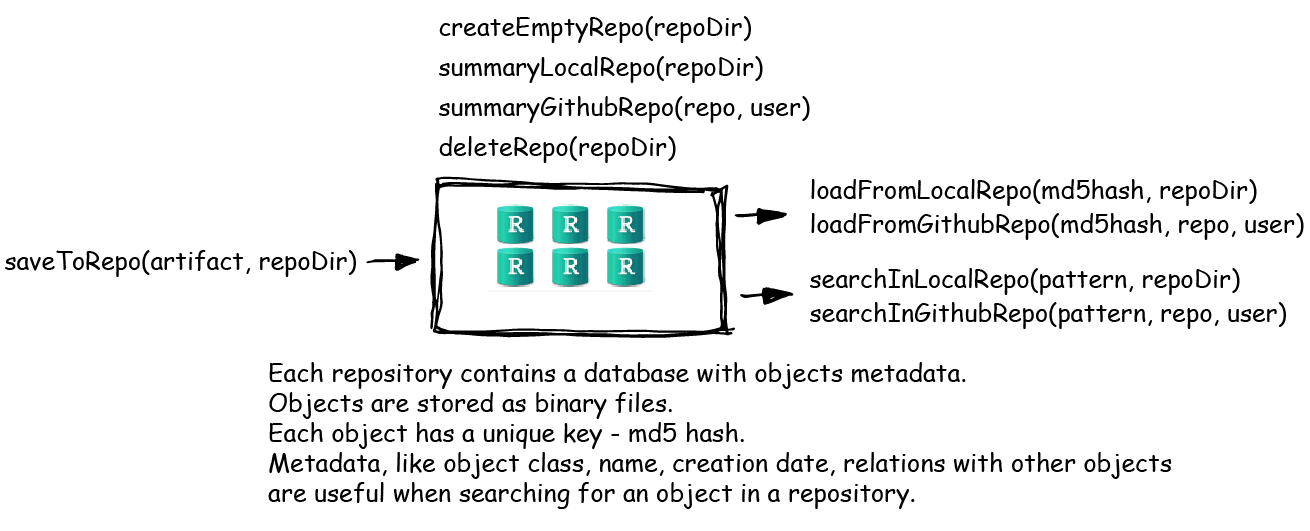
\includegraphics[width=\textwidth]{schemat.png}
  \caption{Schemat pakietu archivist}
\end{figure}

Przedstwaimy działanie tego pakietu na przykładzie wyników naszych badań
genetycznych.

Pakiet archivist jest wzorowany na możliwościach, które daje system
StatLinks wykorzystywany przez w raportach statystycznych.

Kluczowe funkcjonalności tego pakietu opisuje powyższy rysunek. Są to:

\begin{itemize}
\itemsep1pt\parskip0pt\parsep0pt
\item
  Tworzenie/modyfikowanie/usuwanie repozytoriów,
\item
  Dodawanie/usuwanie obiektów oraz ich meta danych z repozytoriów,
\item
  Odczytywanie obiektów z repozytoriów,
\item
  Przeszukiwanie repozytoriów.
\end{itemize}

\textbackslash{}begin\{Schunk\} \textbackslash{}begin\{Sinput\}
library(RTCGA.clinical) library(ggplot2) library(survMisc)
data(``BRCA.clinical'')

clinic \textless{}- data.frame(time1 =
as.numeric(as.character(BRCA.clinical\(patient.days_to_death)),  time2 = as.numeric(as.character(BRCA.clinical\)patient.days\_to\_last\_followup)),
status =
BRCA.clinical\(patient.vital_status,  tumor = substr(BRCA.clinical\)patient.stage\_event.tnm\_categories.pathologic\_categories.pathologic\_t,
1, 2))

clinic\(time <- ifelse(is.na(clinic\)time1),
clinic\(time2, clinic\)time1)

ob1 \textless{}- survfit(Surv(time, status ==
``dead'')\textasciitilde{}tumor, data=clinic) ob2 \textless{}-
autoplot(ob1)\$plot + ylim(0,1) \textbackslash{}end\{Sinput\}
\textbackslash{}end\{Schunk\}

\begin{Schunk}
\begin{Sinput}
ob2
\end{Sinput}

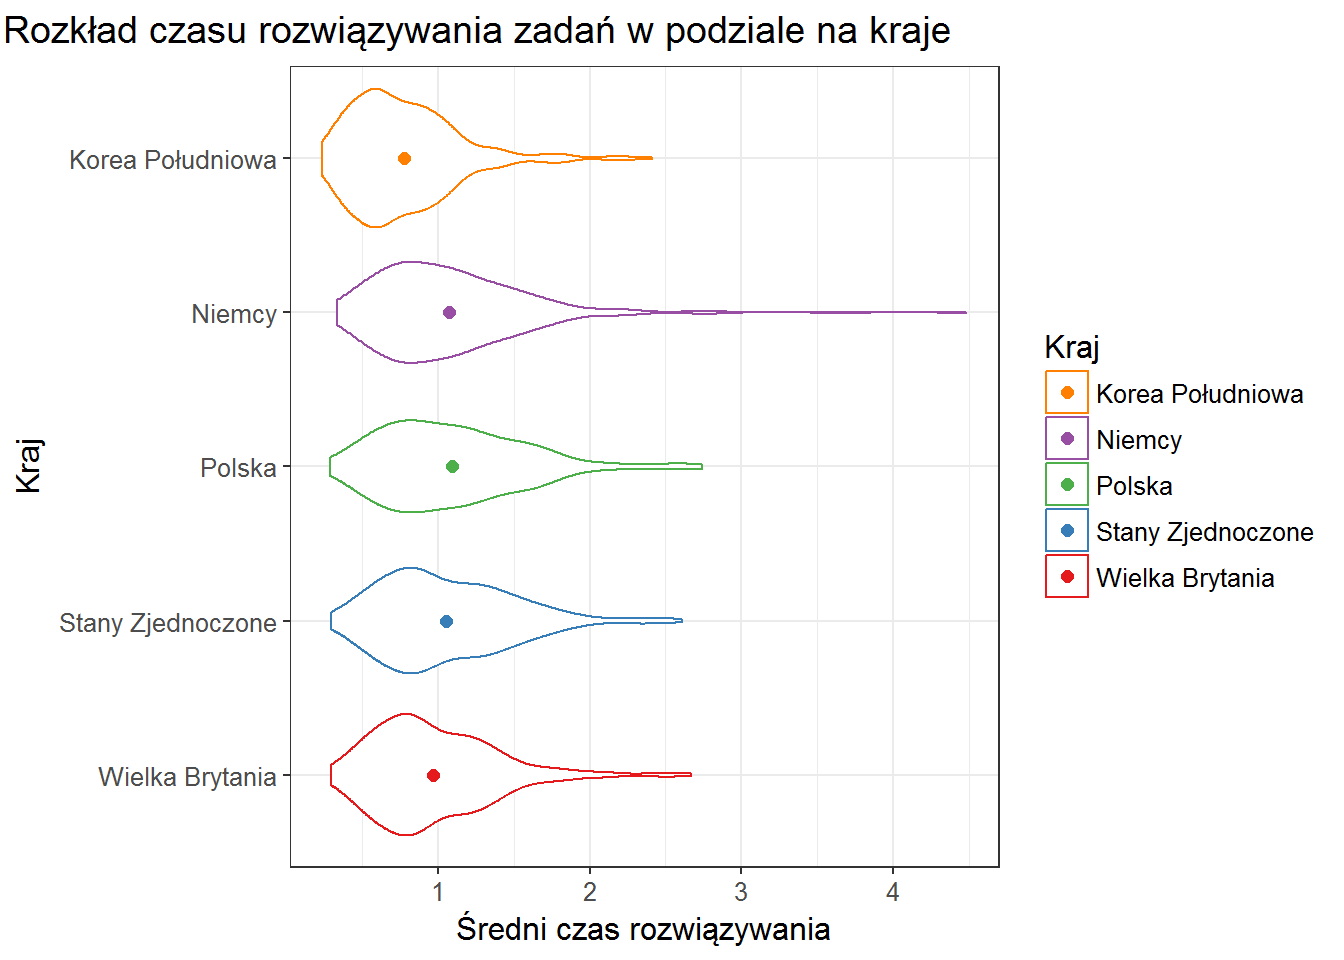
\includegraphics{VolcanoJournal_files/figure-latex/unnamed-chunk-2-1} \end{Schunk}

\subsection{Repozytorium}\label{repozytorium}

Repozytorium może być katalogiem na lokalnym dysku. Repozytorium może
być katalogiem w pakiecie. Repozytorium może być katalogiem na GitHubie.

Zdalne repozytorium

\begin{Schunk}
\begin{Sinput}
library(archivist)
archivist::aread("pbiecek/graphGallery/2a6e492cb6982f230e48cf46023e2e4f")
\end{Sinput}
\end{Schunk}

Pakiet

\begin{Schunk}
\begin{Sinput}
setLocalRepo(repoDir = system.file("graphGallery", package = "archivist"))
archivist::aread("2a6e492cb6982f230e48cf46023e2e4f")
\end{Sinput}
\end{Schunk}

Lokalny katalog

\begin{Schunk}
\begin{Sinput}
library(archivist)
createEmptyRepo("test", default = TRUE)

saveToRepo(ob1)
saveToRepo(ob2)

# odczytaj wartość
loadFromLocalRepo("42ebb8db81d506e94e7a2878f423ded5", value = TRUE)

wykresy <- searchInLocalRepo(pattern = "class:gg")
\end{Sinput}
\end{Schunk}

\citep{R}

\bibliography{RJreferences}

\address{
Przemysław Biecek\\
MiNI Politechnika Warszawska\\
line Koszykowa 75\\ line Warszawa, Polska\\
}
\href{mailto:P.Biecek@mini.pw.edu.pl}{\nolinkurl{P.Biecek@mini.pw.edu.pl}}

